\documentclass{beamer}
\usepackage[utf8]{inputenc}
\usepackage[brazil]{babel}
\usepackage{amsmath}
\usepackage{amsfonts}
\usepackage{amssymb}
\usepackage{fix-cm}
\usepackage{graphicx}
\usepackage{listings}

\usepackage{wrapfig}
\usepackage{indentfirst}
\usepackage{float}
\graphicspath{{recursos/}}

\usetheme{Warsaw}


\title[Trabalho de Gerenciamento de Dados Distribuídos - CI303]{Controle de acesso e \textit{privacy}}
\author[Antonio Carlos, Roger e Tiago.]{Antonio Carlos Salzvedel Furtado Junior, Roger Roberto Rocha Duarte, Tiago Rodrigo Kepe}
\institute{Universidade Federal do Paraná - UFPR}
\date{\today}

\begin{document}

\begin{frame}
\titlepage
\end{frame}

\frame[allowframebreaks]{
	\frametitle{Sumário}
	\tableofcontents
}

\section{Introdução}


\begin{frame}{Motivação}

	\begin{itemize}
	 \item Aplicações colaborativas
	 \item Grids Computacionais
	 \item Redes de Distribuição de conteúdo (CDNs)
	\end{itemize}
\end{frame}

\begin{frame}{Problemas}

	\begin{itemize}
	 \item Peers são igualmente confiáveis
	 \item Quem é dono dos dados?
	\end{itemize}
\end{frame}


\section{Trabalhos relacionados}
\begin{frame}
    \begin{itemize}
      \item Uso de supernodos apra guardar restrições
      \item Criptografia e distribuição de chaves
    \end{itemize}
    \begin{block}{Limitação}
      Escalabilidade
    \end{block}

  \end{frame}

\section{Propostas}

\subsection{Controle de acesso local dos participantes} %% O cara não dá nome pra solução dele.

\begin{frame}{Contexto}
  \begin{itemize}
   \item Peers são estáveis
   \item Replicação não é considerada
   \item Controle de acesso local dos dados e estruturação
   \item Autoridade de certificação centralizada
  \end{itemize}

\end{frame}


\begin{frame}{Componentes}
 \begin{block}{Níveis de funcionamento}
  \begin{itemize}
   \item Nível de peer
   \item Baseado no usuário
  \end{itemize}
 \end{block}
 \begin{figure}[H]
    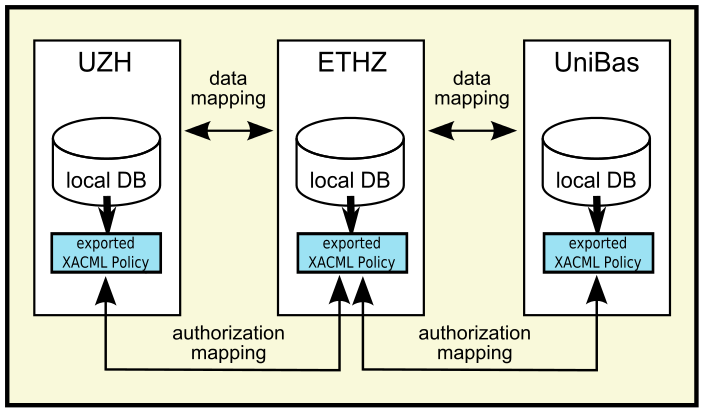
\includegraphics[scale=0.3]{demap_fig1.png}
 \end{figure}

\end{frame}

\begin{frame}[plain]{XACML}
\lstinputlisting[language=xml,basicstyle=\tiny,columns=fullflexible]{recursos/demap_cod1.xml}
\end{frame}

\subsubsection{Política de mapeamento}
  \begin{frame}{Política de mapeamento}
   \begin{figure}[H]
    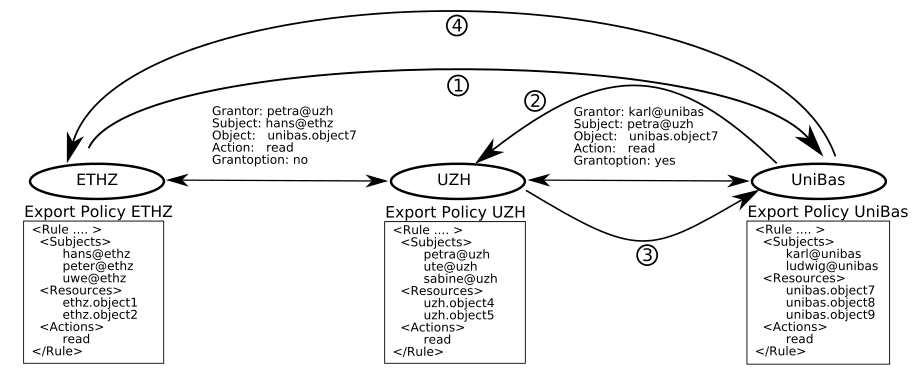
\includegraphics[scale=0.36]{demap_fig2_mp.png}
    \caption{hanz@ethz requisita unibas.object7}
   \end{figure}

  \end{frame}


\subsubsection{Diretório distribuído}
  \begin{frame}{Diretório distribuído}
   \begin{figure}[H]
    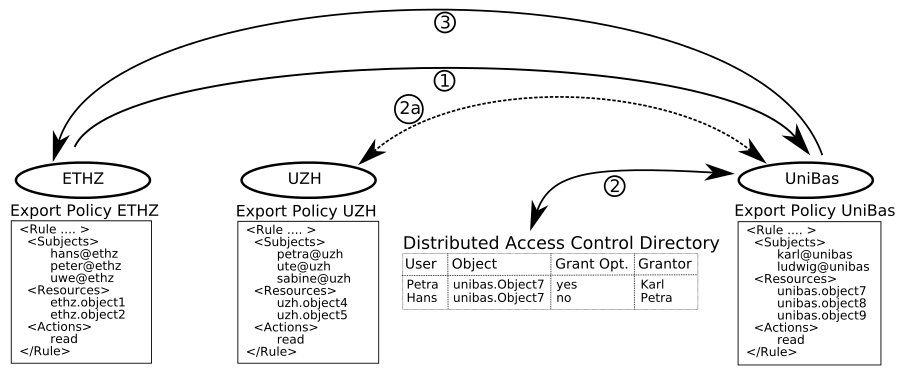
\includegraphics[scale=0.36]{demap_fig3_dd.png}
   \end{figure}

  \end{frame}
  
  \begin{frame}{Diretório distribuído - Implementação}
    \begin{itemize}
     \item Usa-se a DHT
     \item Chord
     \begin{itemize}
      \item \textit{Overhead} para manutenção do diretório
     \end{itemize}

    \end{itemize}

  \end{frame}



\subsection{P-Hera}


\section{Conclusão}


\section{Perguntas}

\begin{frame}{Perguntas}
	\begin{center}		
		\Huge PERGUNTAS?
	\end{center}
	
\end{frame}
\end{document}
